\chapter{Week 5}
\section{ARMA Parameter Estimation: AR Case}
Suppose we observe a time series
$ X_1,\ldots,X_T \sim \ARMA{p,q} $
\[ \phi(B)X_t=\theta(B)X_t \]
\[ \phi(z)=1-\phi_1 z-\cdots - \phi_p z^p \]
\[ \theta(z)=1+\theta_1 z+\cdots+\theta_q z^q \]
Our goal is to estimate
\begin{itemize}
    \item $ \phi_1,\ldots,\phi_p $ (AR parameters)
    \item $ \theta_1,\ldots,\theta_q $ (MA parameters)
    \item $ \sigma_W^2 $ (white noise variance)
\end{itemize}
$ \AR{1} $ case: $ X_t=\phi X_{t-1}+W_t $ with $ \E{W_t^2}=\sigma_W^2 $.
The idea is to use OLS\@.
\[ \hat{\phi}=\argmin_{\abs{\phi}<1}\sum_{t=2}^{T} (X_t-\phi X_{t-1})^2 \]
This leads to (upon some calculations):
\[ \hat{\phi}=\frac{\frac{1}{T}  \sum_{t=2}^{T} X_t X_{t-1}}{\frac{1}{T} \sum_{t=2}^{T} X_t^2}
    \approx \frac{\hat{\gamma}(1)}{\hat{\gamma}(0)}=\hat{\rho}(1)
    \xrightarrow[T\to\infty]{P}\phi   \]
\[ \hat{\sigma}_W^2=\frac{1}{T-1} \sum_{t=2}^{T} (X_t-\hat{\phi}X_{t-1})^2 \]
where $ X_t-\hat{\phi}X_{t-1} $ is estimated $ W_t $ and $ \hat{\sigma}_W^2 $
is the sample variance of residuals.

$ \AR{p} $ case: $ X_t=\phi_1 X_{t-1}+\cdots+\phi_p X_{t-p}+W_t $.
OLS\@: $ \symbf{\phi}=(\phi_1,\ldots,\phi_p)^\top \in\mathbf{R}^p $
\[ \hat{\symbf{\phi}}=\argmin_{\hat{\symbf{\phi}}}\sum_{t=p+1}^{T} (X_t-\phi_1X_{t-1}-\cdots-\phi_p X_{t-p})^2 \]
$\hat{\symbf{\phi}}$ admits a stationary and causal solution.

Solve using calculus (take first order partial derivatives set equal to zero),
leads to a system of $ p $ linear equations of the form
\[ \hat{\Gamma}_p \symbf{\hat{\phi}}=\hat{\symbf{\gamma}_p} \]
where
\[ \hat{\Gamma}_p=(\hat{\gamma}(j-k),\, 1\le j,k\le p)\in\mathbf{R}^{p\times p} \]
\[ \symbf{\hat{\gamma}}_p=(\hat{\gamma}(1).\ldots,\hat{\gamma}(p))^\top \]
The resulting OLS estimator takes the form
\[ \hat{\symbf{\phi}}=\hat{\Gamma}_p^{-1}\hat{\symbf{\gamma}}_p \]
\[ \hat{\sigma}_W^2=\hat{\gamma}(0)-\hat{\symbf{\gamma}}_p^\top \hat{\Gamma}_p \hat{\symbf{\gamma}}_p \]
Similar approach: use method of moments (set parameters so that
empirical moments match theoretical causal moments induced by the model).

If $ X_t \sim \AR{p} $, then for $ 1\le h\le p $.
\begin{align*}
    \gamma(h)
     & =\E{X_{t}X_{t+h}}                                               \\
     & =\E{X_t(\phi_1 X_{t+h-1}+\cdots+\phi_p X_{t+h-p}+W_{t+h})}      \\
     & =\phi_1\gamma(h-1)+\phi_2\gamma(h-2)+\cdots+\phi_p\gamma(h-p)+0
\end{align*}
where the $ 0 $ occurs since $ X_t\indep W_{t+h} $.

This implies the linear system:
\[ \symbf{\gamma}_p=\Gamma_p \symbf{\phi} \]
\[ \symbf{ \gamma}_p=(\gamma(1),\ldots,\gamma(p))^\top \in\mathbf{R}^p \]
\[  \Gamma_p=\bigl[\gamma(j-k),\, 1\le j,k\le p\bigr]\in\mathbf{R}^{p\times p} \]
Note that $ X_t=\sum_{\ell=0}^{\infty} \psi_\ell W_{t-\ell} $ where $ \psi_0=1 $
and $ W_t=X_t-\phi_1X_{t-1}-\cdots-\phi_p X_{t-p} $ imply
\[ \sigma_W^2=\E{X_t W_t}
    =\E{X_t(X_t-\phi_1 X_{t-1}-\cdots-\phi_p X_{t-p})}
    =\gamma(0)-\phi_1\gamma(1)-\cdots-\phi_p\gamma(p) \]
which are \textbf{Yule-Walker Equations}.
\[ \symbf{\gamma}_p=\Gamma_p \symbf{\phi} \]
\textbf{Yule-Walker Estimators}:
\[ \hat{\symbf{\phi}}=\hat{\Gamma}_p^{-1} \symbf{\hat{\gamma}}_p \]
\[ \hat{\sigma}_W^2=\hat{\gamma}(0)-\hat{\symbf{\gamma}}_p^\top \hat{\Gamma}_p^{-1}\hat{\symbf{\gamma}}_p \]
\begin{Example}{}{}
    In the $ \AR{1} $ case, the YW estimators are
    \[ \hat{\phi}=\frac{\hat{\gamma}(1)}{\hat{\gamma}(0)}=\hat{\rho}(1)  \]
    \[ \hat{\sigma}_W^2=\hat{\gamma}(0)-\frac{\hat{\gamma}^2(1)}{\hat{\gamma}(0)}  \]
\end{Example}
\begin{Theorem}{}{}
    If $ X_t \sim \AR{p} $ (causal), then
    \[ \frac{\hat{\phi}_{\text{OLS, $i$}}}{\hat{\phi}_{\text{YW, $i$}}}
        \xrightarrow[T\to\infty]{P}1  \]
    OLS and YW estimates are asymptotically equivalent.
\end{Theorem}
\begin{Theorem}{}{}
    \[ \sqrt{T}\bigl(\hat{\symbf{\phi}}_{\text{YW}}-\symbf{\phi}\bigr)
        \xrightarrow[T\to\infty]{D}\Mvn{0,\sigma_W^2\Gamma_p^{-1}} \]
    \[ \hat{\sigma}_W^2\xrightarrow{P}\sigma_W^2 \]
    \begin{itemize}
        \item Optimal variance among all possible (asymptotically) unbiased estimators, hence \textbf{efficient}.
        \item Result can be used to obtain confidence intervals for $ \phi $.
    \end{itemize}
\end{Theorem}

\section{ARMA Parameter Estimation: MLE}
Ordinary Least Squares and Yule-Walker equation
estimators are effective in estimating the $ \AR{p} $
parameters, but are difficult to apply to fitting
$ \MA{q} $ and general $ \ARMA{p,q} $
models since the white noises $ W_t $ are not observable,
and YW equations are not linear in the MA parameters.

Latent Variables (variables associated with $ W_t $) $\implies$
MLE is best.

Suppose $ X_t \sim \AR{1} $ (causal)
\[ X_t=\phi X_{t-1}+W_t \]
where $ W_t \stackrel{\text{iid}}{\sim}\N{0,\sigma_W^2} $,
then
\[ X_t=\sum_{\ell=0}^{\infty} \phi^\ell W_{t-\ell} \]
is Gaussian. $ L^2 $ limits of Gaussian random variables are Gaussian.
(MGF or characteristic function).

Moreover, $ X_1,\ldots,X_T $ are jointly Gaussian since
\[ a_1X_1+\cdots+a_T X_T= \sum_{\ell=0}^{\infty}
    \phi^\ell (\Uunderbracket{a_1 W_{1-\ell}+\cdots+a_T W_{t-\ell}}_{\text{Gaussian}}) \]
MLE\@:
\[ \mathcal{L}(\phi,\sigma_W^2)=f(X_T, X_{T-1},\ldots,X_1;\phi,\sigma_W^2) \]
where
\begin{itemize}
    \item $\mathcal{L}(\phi,\sigma_W^2)$ is the likelihood of $ \phi $ and $ \sigma_W^2 $.
    \item $f(X_T, X_{T-1},\ldots,X_1;\phi,\sigma_W^2)$ is the joint density
          of $ X_T,\ldots,X_1 $ at the observed data. Gaussian Density.
\end{itemize}
Key idea in Time series: To evaluate the likelihood condition on
the path/past!
\begin{align*}
    f(X_T,\ldots,X_1)
     & =f(X_T\mid X_{T-1},\ldots,X_1)f(X_{T-1},\ldots,X_1)                                                            \\
     & \vdotswithin{=}                                                                            &  & \text{iterate} \\
     & =f(X_T\mid X_{T-1},\ldots,X_1)f(X_{T-1}\mid X_{T-2},\ldots,X_1)\cdots f(X_2\mid X_1)f(X_1)                     \\
     & =\prod_{i=1}^T f(X_i\mid X_{i-1},\ldots,X_1)
\end{align*}
According to HW2:
\[ X_i \mid (X_{i-1},\ldots,X_1)\sim \N{\phi X_{i-1},\sigma_W^2} \]
Note that $  X_i \mid (X_{i-1},\ldots,X_1)=X_i\mid X_{i-1} $, $ \AR{1} $.

Thus,
\begin{align*}
    \mathcal{L}(\phi,\sigma_W^2)
     & = \prod_{i=2}^T \frac{1}{\sqrt{2\pi\sigma_W^2}}\expon*{-\frac{(X_i-\phi X_{i-1})^2}{2\sigma_W^2} }f(X_1)                   \\
     & = (2\pi\sigma_W^2)^{-\frac{T-1}{2}}\expon*{-\frac{\sum_{i=2}^{T} (X_i-\phi X_{i-1})^2}{2\sigma_W^2}}f(X_1;\phi,\sigma_W^2)
\end{align*}
Maximizing $ \mathcal{L}(\phi,\sigma_W^2) $ in this case leads to a similar estimator as OLS/YW\@.

General $ \ARMA{p,q} $ case: Again, $ X_T,\ldots,X_1 $ are jointly
Gaussian if $ W_t \sim  $ Gaussian.
\[ L(\Uunderbracket{\phi_1,\ldots,\phi_p,\theta_1,\ldots,\theta_q,\sigma_W^2}_{\symbf{\theta}\in\mathbf{R}^{p+q+1}})=
    \prod_{i=1}^T \Uunderbracket{f(X_i\mid X_{i-1},\ldots,X_1)}_{\text{Gaussian}} \]
\begin{align*}
    X_i\mid (X_{i-1},\ldots,X_1)
     & \sim \N[\big]{\E{X_i\given X_{i-1},\ldots,X_1},\text{MSE}}                       \\
     & \sim \N[\big]{\tilde{X}_{i\mid (i-1)}(\symbf{\theta}),P_{i-1}^i(\symbf{\theta})}
\end{align*}
where $ P_{i-1}^i(\symbf{\theta}) $ is forecast MSE predicting $ X_i $ from $ X_{i-1},\ldots,X_1 $.

This likelihood can be maximized using numerical optimization. (Newton-Raphson Algorithm,
Conjugate Gradient).

\begin{Theorem}{Chapter 8 of Brockwell and Davis, Hannan (1980)}{}
    The MLE's of $ \phi_1,\ldots,\phi_p,\theta_1,\ldots,\theta_q,\sigma_W^2 $
    are $ \sqrt{T} $ consistent and asymptotically Normal with asymptotic covariance
    equal to the inverse of the information matrix. In this sense, they
    are asymptotically optimal.
\end{Theorem}
\begin{Remark}{Takeaway Message}{}
    \begin{enumerate}[(1)]
        \item MLE estimation reduces to OLS, YW equation estimation for $ \AR{p} $ models.
        \item For general $ \ARMA{p,q} $ estimation, MLE
              is through to be optimal in most situations. (Used as a default/benchmark).
    \end{enumerate}
\end{Remark}

\section{Model Selection Diagnostic Tests}
Using MLE, we can fit an $ \ARMA{p,q} $
model to an observed series $ X_1,\ldots ,X_T $.

Question: How do we select the orders $ p $ and $ q $ of the model?
\subsection*{Usual Methods}
\begin{enumerate}[(1)]
    \item Examine ACF and PACF\@.
    \item Model Diagnostics/Goodness-of-Fit tests:
          Examine the residuals of the $ \ARMA{p,q} $ model to check for the plausibility
          of the white noise assumption.
    \item Model Selection Methods: Information criteria, cross-validation.
\end{enumerate}
\subsection*{Model Diagnostics}
If the $ \ARMA{p,q} $ model fits the data well, then the estimated residuals
should behave like white noise.
\[ \hat{W}_{t}=\frac{X_t-\tilde{X}_{t\mid (t-1)}}{\sqrt{\hat{P}^{t-1}_{t}}}  \]
where
\begin{itemize}
    \item $ \tilde{X}_{t\mid(t-1)} $ is the truncated predicator of $ X_t $
          based on $ X_{t-1},\ldots,X_1 $, and
    \item $ \hat{P}_t^{t+1} $ is the estimated MSE\@.
\end{itemize}
This can be investigated by considering
$ \hat{\rho}_W(h) $
which is the empirical ACF of $ \hat{W}_1,\ldots,\hat{W}_T $.

As a measure of how ``white'' the residuals are, it is common
to evaluate the cumulative significance of $ \hat{\rho}_W(h) $
for $ 1\le h\le H $ by applying a ``white noise test.''
Suppose $ W_1,\ldots,W_T $ is a strong white noise, and
$ \hat{\rho}_W(h) $ is the empirical ACF of this series.

We know that for each fixed $ h $,
\[ \sqrt{T}\hat{\rho}_W(h)\xrightarrow{D}\N{0,1} \]
Also, for $ j\ne h $,
\begin{align*}
    \Cov[\big]{\sqrt{T}\hat{\gamma}_W(h),\sqrt{T}\hat{\gamma}_W(j)}
     & =T\E*{\sum_{t=1}^{T} W_t W_{t+h}}\E*{\sum_{s=1}^{T} W_s W_{s+j}} \\
     & =T \sum_{t=1}^{T} \sum_{s=1}^{T} \E{W_{t}W_{t+h}W_{s}W_{s+j}}    \\
     & =0
\end{align*}
Using Martingale, or $ m $-dependent CLT's, it can be shown that
\[ \begin{pmatrix}
        \sqrt{T}\hat{\rho}_W(1) \\
        \vdots                  \\
        \sqrt{T}\hat{\rho}_W(H)
    \end{pmatrix}
    \xrightarrow{D} \Mvn{0,I_{H\times H}} \]
Therefore,
\[ T \sum_{h=1}^{H} \hat{\rho}_W^2(h)
    \xrightarrow{D}\chi^2(H) \]

\subsection*{Box-Ljung-Pierce Test [White Noise Test for $ \ARMA{p,q} $ Models]}
If $ X_t \sim \ARMA{p,q} $, and $ \hat{W}_t $ are the model residuals
with empirical ACF $ \hat{\rho}_W(h) $, then if
\[ Q(T,H)=T(T+2)\sum_{h=1}^{H} \frac{\hat{\rho}_W^2(h)}{T-h}\approx
    T \sum_{h=1}^{H} \hat{\rho}_W^2(h)  \]
\[ Q(T,H)\xrightarrow[T\to\infty]{D}\chi^2(H-(p+q)) \]
That is, we lose $ p+q $ degrees of freedom for fitting the model.

The BLP test $ p $-value is then computed as
\[ P_{\text{BLP}}=\Prob[\big]{\chi^2(H-(p+q))>Q(T,H)} \]

\begin{Remark}{}{}
    If $ X_t \sim \ARMA{p,q} $, and $ \hat{W}_t $
    are calculated based on $ \ARMA{p^\prime,q^\prime} $ model
    where $ p^\prime <p $ or $ p^\prime <q $ (model is under specified),
    then
    \[ Q(T,H)\xrightarrow[T\to\infty]{P}\infty \]
    \underline{Interpretation}: If BLP $ p $-values are small,
    the model is ill-fitting or under specified.
\end{Remark}

\section{Model Selection Information Criteria}
Suppose we are trying to select the orders $ p $ and
$ q $ of an $ \ARMA{p,q} $ model to fit $ X_1,\ldots,X_T $.
\[ \symbf{\phi}=\text{AR parameters} \]
\[ \symbf{\theta}=\text{MA parameters} \]
\[ \sigma_W^2=\text{white noise variance} \]
\[ \mathcal{L}(X_1,\ldots,X_T;\hat{\symbf{\phi}},\hat{\symbf{\theta}},\sigma_W^2) \]
Natural idea: Maximize the likelihood of the data as a function of
$ p $ and $ q $.

\underline{Problem}: The likelihood is (monotonically)
increasing as a function of $ p $ and $ q $. Maximizing would lead
to overfitting.

\underline{Solution}: Maximize the likelihood subject to a
penalty term on the number of parameters (complexity)
of the model. Let the number of parameters
in the $ \ARMA{p,q} $ model be denoted by $ k=p+q+1 $.
\[ -2\log*{\mathcal{L}(X_1,\ldots,X_T;\hat{\symbf{\phi}},\hat{\symbf{\theta}},\sigma_W^2)}+P(T,k) \]
where $ P(T,k) $ is an increasing function of $ k $.

Optimal $ p $ and $ q $ balance model fit with the penalty for complexity.

\subsection*{Common Penalty Term Choices}
\begin{itemize}
    \item $ \AIC{p,q}=-2\log*{\mathcal{L}(X_1,\ldots,X_T;\hat{\symbf{\phi}},\hat{\symbf{\theta}},\sigma_W^2)}+\dfrac{2k+T}{T} $.
          \begin{itemize}
              \item Comes from estimating the Kullback–Leibler distance from the fitted model to the ``true'' model.
          \end{itemize}
    \item $ \BIC{p,q}=-2\log*{\mathcal{L}(X_1,\ldots,X_T;\hat{\symbf{\phi}},\hat{\symbf{\theta}},\sigma_W^2)}+\dfrac{k\log{T}}{T} $.
          \begin{itemize}
              \item Comes from approximating and maximizing the posterior distribution of the model given the data.
          \end{itemize}
\end{itemize}
\underline{Interpretation}: Small AIC/BIC mean a better model.

Information criteria are also used in trend fitting. Suppose
\[ X_t=s_t+Y_t=f_t(\symbf{\beta})+Y_t \]
where $ \symbf{\beta}\in\mathbf{R}^k $ and $ f_t(\symbf{\beta}) $ is the trend we fit.

Estimate $ \symbf{\beta} $ with $ \hat{\symbf{\beta}} $ using ordinary least squares.
\[ \SS{Res}_T=\sum_{t=1}^{T}(X_t-f_t(\symbf{\hat{\beta}}))^2 \]
Information criteria typically calculated assuming $ Y_t $ is a Gaussian white noise.
\[ \SS{Res}_T+P(T,k) \]
where for $ P(T,k) $ we use AIC or BIC penalty.
\begin{Remark}{}{}
    \begin{enumerate}[(1)]
        \item In trend fitting, the assumption of Gaussian white noise residuals is often in doubt.
        \item AIC/BIC are not perfect! They are but one of many tools useful in model selection.

              \textbf{Strengths}:
              \begin{enumerate}[(i)]
                  \item Easy to compute.
                  \item Facilitates comparing many models quickly.
              \end{enumerate}
              \textbf{Weaknesses}:
              \begin{enumerate}[(i)]
                  \item Likelihood must be specified.
                  \item There is a degree of ``arbitrariness'' to the choice of penalty.
              \end{enumerate}
        \item It can be shown that minimizing the AIC is related to minimizing
              the $ 1 $-step forecast MSE, and so when the application is forecasting,
              AIC is more common.
    \end{enumerate}
\end{Remark}
\section{ARIMA Models}
We have seen that many time series appear stationary after differencing.
\begin{Definition}{Integrated}{}
    We say a time series $ X_t $ is \textbf{integrated} to order $ d $
    if $ \nabla^d X_t $ is stationary, but $ \nabla^j X_t $
    for $ 1\le j\le d $ is \underline{not} stationary.
\end{Definition}
\underline{Motivation}: If $ Y_t $ is stationary,
and $ X_t=\sum_{j=1}^{t} Y_j $, $ X_t $ is integrated to order 1.
$ Z_t=\sum_{j=1}^{t} X_j $ is integrated to order 2, and so on.
\begin{Definition}{ARIMA}{}
    We say $ X_t $ follows an \textbf{Autoregressive Integrated Moving Average Process}
    (ARIMA) of orders $ p,d,q $ if
    \[ \phi(B)(1-B)^d X_t=\theta(B)W_t \]
    and write $ X_t \sim \ARIMA{p,d,q} $. Note that $ \nabla^d X_t $
    follows an $ \ARMA{p,q} $ model.
\end{Definition}
\subsection*{Forecasting $ \ARIMA{p,d,q} $ Processes}
\begin{enumerate}[(1)]
    \item $ Y_t=\nabla^d X_t $ follows an $ \ARMA{p,q} $ model
          and so can be forecast using truncated ARMA prediction.
    \item Forecasts $ \hat{Y}_{T+h\mid T} $ can be used to forecast $ X_{T+h} $
          by reversing the differencing.
          \begin{Example}{}{}
              For $ d=1 $, $ Y_{T+1}=X_{T+1}-X_{T} $ so $ \hat{X}_{T+1\mid T}=X_T+\hat{Y}_{T+1\mid T} $.
              This can be iterated to produce longer Horizon forecasts.
          \end{Example}
\end{enumerate}
Predicting MSE is approximately of the form
\[ P_{T+h}^T\approx \sigma_W^2 \sum_{j=0}^{h-1} \psi^2_{j,*} \]
where $  \psi^2_{j,*} $ is the coefficient of $ z^j $ in the
power series expansion (centred at zero) of
\[ \frac{\theta(z)}{\phi(z)(1-z)^d} \quad(\abs{z}<1) \]
Idea:
\[ X_t \approx \frac{\theta(B)}{\phi(B)(1-B)^d}W_t  \]
\begin{Example}{}{}
    Let $ X_t \sim \ARIMA{0,1,0} $.
    \[ X_t-X_{t-1}=(1-B)X_t=W_t\implies X_t=X_{t-1}+W_t\implies X_t=\sum_{j=1}^{t} W_j \]
    if we iterate $ t $-times. If $ Y_t = \nabla X_t $, then $ \hat{Y}_{T+h\mid T}=0 $
    (forecasting $ W_t $'s). Therefore,
    \[ \hat{X}_{T+1\mid T}=X_t+\hat{Y}_{T+1\mid T}=X_T \]
    Similarly, $ \hat{X}_{T+h\mid T}=X_T $. The best predictor of random walk is last known location.

    Prediction MSE\@: \[ \frac{\theta(z)}{\phi(z)(1-z)^d}=\frac{1}{1-z} =\sum_{j=0}^{\infty} z^j\quad(\abs{z}<1)  \]
    \begin{align*}
         & \implies\psi_{j,*}=1\quad(\forall j)                                    \\
         & \implies P_{T+h}^T=\sigma_W^2 \sum_{j=0}^{h-1} \psi_{j,*}^2=h\sigma_W^2
    \end{align*}
    Note that
    \[ \E*{(\hat{X}_{T+h\mid T}-X_{T+h})^2}=\E*{\biggl(\sum_{j=T+1}^{T+h} W_j\biggr)^2}=h\sigma_W^2 \]
    \begin{center}
        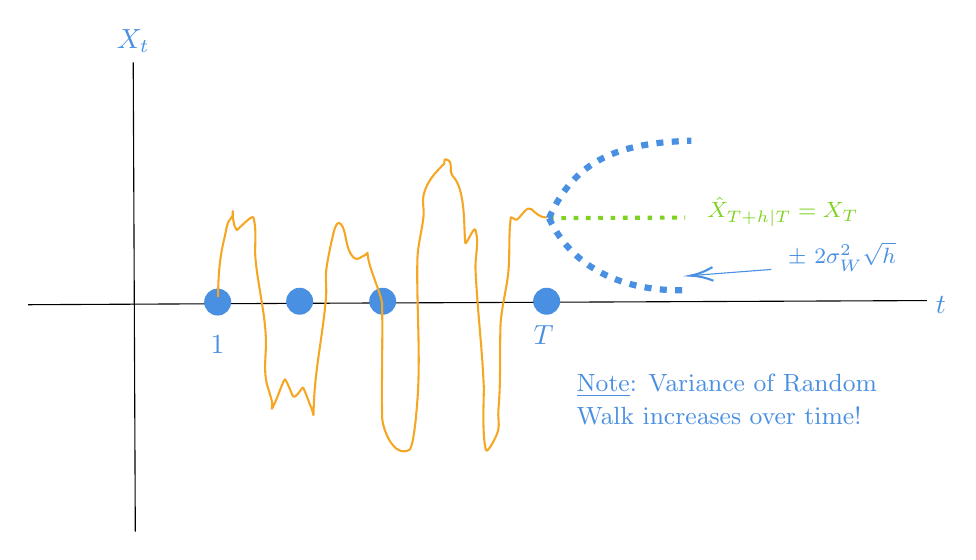
\begin{tikzpicture}[x=0.75pt,y=0.75pt,yscale=-1,xscale=1]
            %uncomment if require: \path (0,300); %set diagram left start at 0, and has height of 300

            %Straight Lines [id:da9553447572143613] 
            \draw    (1.1,141.7) -- (134.37,141.02) -- (434.1,139.7) ;
            %Straight Lines [id:da06218855892004649] 
            \draw    (52.69,251) -- (51.69,25) ;
            %Shape: Circle [id:dp6867683503986474] 
            \draw  [draw opacity=0][fill={rgb, 255:red, 74; green, 144; blue, 226 }  ,fill opacity=1 ] (85.87,140.42) .. controls (85.87,136.83) and (88.78,133.93) .. (92.37,133.93) .. controls (95.95,133.93) and (98.86,136.83) .. (98.86,140.42) .. controls (98.86,144.01) and (95.95,146.92) .. (92.37,146.92) .. controls (88.78,146.92) and (85.87,144.01) .. (85.87,140.42) -- cycle ;
            %Shape: Circle [id:dp6098097598249137] 
            \draw  [draw opacity=0][fill={rgb, 255:red, 74; green, 144; blue, 226 }  ,fill opacity=1 ] (125.38,140.02) .. controls (125.38,136.43) and (128.28,133.53) .. (131.87,133.53) .. controls (135.46,133.53) and (138.37,136.43) .. (138.37,140.02) .. controls (138.37,143.61) and (135.46,146.52) .. (131.87,146.52) .. controls (128.28,146.52) and (125.38,143.61) .. (125.38,140.02) -- cycle ;
            %Shape: Circle [id:dp12857612146858388] 
            \draw  [draw opacity=0][fill={rgb, 255:red, 74; green, 144; blue, 226 }  ,fill opacity=1 ] (165.38,140.02) .. controls (165.38,136.43) and (168.28,133.53) .. (171.87,133.53) .. controls (175.46,133.53) and (178.37,136.43) .. (178.37,140.02) .. controls (178.37,143.61) and (175.46,146.52) .. (171.87,146.52) .. controls (168.28,146.52) and (165.38,143.61) .. (165.38,140.02) -- cycle ;
            %Shape: Circle [id:dp37098830977149844] 
            \draw  [draw opacity=0][fill={rgb, 255:red, 74; green, 144; blue, 226 }  ,fill opacity=1 ] (244.38,140.02) .. controls (244.38,136.43) and (247.28,133.53) .. (250.87,133.53) .. controls (254.46,133.53) and (257.37,136.43) .. (257.37,140.02) .. controls (257.37,143.61) and (254.46,146.52) .. (250.87,146.52) .. controls (247.28,146.52) and (244.38,143.61) .. (244.38,140.02) -- cycle ;
            %Shape: Free Drawing [id:dp2306557468398488] 
            \draw  [color={rgb, 255:red, 245; green, 166; blue, 35 }  ,draw opacity=1 ][line width=0.75] [line join = round][line cap = round] (92.6,137.7) .. controls (92.6,128.31) and (93.32,118.81) .. (95.6,109.7) .. controls (96.38,106.59) and (96.59,103.71) .. (97.6,101.7) .. controls (98.14,100.63) and (99.15,99.82) .. (99.6,98.7) .. controls (99.85,98.08) and (99.6,96.03) .. (99.6,96.7) .. controls (99.6,99.27) and (99.98,104.08) .. (101.6,105.7) .. controls (101.8,105.9) and (109.12,97.96) .. (109.6,99.7) .. controls (111.39,106.13) and (110,113.05) .. (110.6,119.7) .. controls (111.73,132.08) and (115.1,145.1) .. (115.6,157.7) .. controls (115.92,165.7) and (114.07,174.1) .. (116.6,181.7) .. controls (117.28,183.75) and (118.13,186.81) .. (118.6,188.7) .. controls (118.84,189.67) and (118.12,192.58) .. (118.6,191.7) .. controls (121.03,187.24) and (122.33,182.24) .. (124.6,177.7) .. controls (125.11,176.68) and (128.25,185.23) .. (128.6,185.7) .. controls (129.96,187.51) and (133.17,180.84) .. (133.6,181.7) .. controls (135.21,184.91) and (136.11,188.43) .. (137.6,191.7) .. controls (138.04,192.66) and (138.6,195.75) .. (138.6,194.7) .. controls (138.6,175.09) and (143.13,156.87) .. (144.6,137.7) .. controls (144.91,133.71) and (144.27,129.69) .. (144.6,125.7) .. controls (144.82,123.01) and (146.46,114.25) .. (147.6,109.7) .. controls (147.83,108.8) and (149.24,100.34) .. (151.6,102.7) .. controls (154.56,105.66) and (153.7,114.8) .. (157.6,118.7) .. controls (159.92,121.02) and (161.01,118.56) .. (163.6,117.7) .. controls (164.05,117.55) and (164.6,116.23) .. (164.6,116.7) .. controls (164.6,123.12) and (171.51,136.67) .. (171.6,141.7) .. controls (171.93,159.7) and (171.27,177.7) .. (171.6,195.7) .. controls (171.7,201.47) and (177.04,215.48) .. (184.6,211.7) .. controls (187.03,210.48) and (188.45,189.66) .. (188.6,187.7) .. controls (190.26,166.07) and (188.09,141.42) .. (188.6,119.7) .. controls (188.76,112.96) and (191.03,105) .. (191.6,98.7) .. controls (191.9,95.38) and (190.75,91.92) .. (191.6,88.7) .. controls (193.48,81.54) and (197.79,77.51) .. (201.6,73.7) .. controls (201.83,73.47) and (201.04,71.18) .. (202.6,71.7) .. controls (206.64,73.05) and (203.17,77.27) .. (205.6,79.7) .. controls (211.71,85.81) and (210.97,102.88) .. (211.6,111.7) .. controls (211.79,114.3) and (215.83,103.21) .. (216.6,105.7) .. controls (218.46,111.75) and (216.32,118.37) .. (216.6,124.7) .. controls (217.43,143.71) and (219.88,163.05) .. (220.6,181.7) .. controls (220.74,185.3) and (219.56,203.53) .. (221.6,211.7) .. controls (221.94,213.07) and (223.91,209.94) .. (224.6,208.7) .. controls (225.83,206.48) and (227.13,204.2) .. (227.6,201.7) .. controls (228.15,198.75) and (227.33,195.69) .. (227.6,192.7) .. controls (228.81,179.42) and (228.27,166.03) .. (228.6,152.7) .. controls (228.83,143.4) and (232.02,133.05) .. (232.6,123.7) .. controls (233.14,115.03) and (232.56,108) .. (233.6,99.7) .. controls (233.69,98.99) and (235.94,101.23) .. (236.6,100.7) .. controls (238.84,98.91) and (241.57,93.67) .. (243.6,95.7) .. controls (245.5,97.6) and (247.91,99.7) .. (250.6,99.7) ;
            %Straight Lines [id:da7457104921148514] 
            \draw [color={rgb, 255:red, 126; green, 211; blue, 33 }  ,draw opacity=1 ][line width=1.5]  [dash pattern={on 1.69pt off 2.76pt}]  (252,100) -- (317.6,99.7) ;
            %Curve Lines [id:da4312930461611998] 
            \draw [color={rgb, 255:red, 74; green, 144; blue, 226 }  ,draw opacity=1 ][line width=2.25]  [dash pattern={on 2.53pt off 3.02pt}]  (252,100) .. controls (264.6,71.7) and (285.6,63.7) .. (320.6,62.7) ;
            %Curve Lines [id:da22250777837248648] 
            \draw [color={rgb, 255:red, 74; green, 144; blue, 226 }  ,draw opacity=1 ][line width=2.25]  [dash pattern={on 2.53pt off 3.02pt}]  (252,100) .. controls (264.6,126.7) and (291.6,135.7) .. (319.6,134.7) ;
            %Straight Lines [id:da8288377199810669] 
            \draw [color={rgb, 255:red, 74; green, 144; blue, 226 }  ,draw opacity=1 ]   (359.1,124.7) -- (322.09,127.55) ;
            \draw [shift={(320.1,127.7)}, rotate = 355.6] [color={rgb, 255:red, 74; green, 144; blue, 226 }  ,draw opacity=1 ][line width=0.75]    (10.93,-3.29) .. controls (6.95,-1.4) and (3.31,-0.3) .. (0,0) .. controls (3.31,0.3) and (6.95,1.4) .. (10.93,3.29)   ;

            % Text Node
            \draw (51.69,21.6) node [anchor=south] [inner sep=0.75pt]  [color={rgb, 255:red, 74; green, 144; blue, 226 }  ,opacity=1 ]  {$X_{t}$};
            % Text Node
            \draw (249.37,150.33) node [anchor=north] [inner sep=0.75pt]  [color={rgb, 255:red, 74; green, 144; blue, 226 }  ,opacity=1 ]  {$T$};
            % Text Node
            \draw (92.37,155.33) node [anchor=north] [inner sep=0.75pt]  [color={rgb, 255:red, 74; green, 144; blue, 226 }  ,opacity=1 ]  {$1$};
            % Text Node
            \draw (437.1,141.7) node [anchor=west] [inner sep=0.75pt]  [color={rgb, 255:red, 74; green, 144; blue, 226 }  ,opacity=1 ]  {$t$};
            % Text Node
            \draw (366,110.4) node [anchor=north west][inner sep=0.75pt]  [font=\footnotesize,color={rgb, 255:red, 74; green, 144; blue, 226 }  ,opacity=1 ]  {$\pm \ 2\sigma ^{2}_{W}\sqrt{h}$};
            % Text Node
            \draw (327,88.4) node [anchor=north west][inner sep=0.75pt]  [font=\footnotesize,color={rgb, 255:red, 126; green, 211; blue, 33 }  ,opacity=1 ]  {$\hat{X}_{T+h\mid T} =X_{T}$};
            % Text Node
            \draw (264,174) node [anchor=north west][inner sep=0.75pt]  [color={rgb, 255:red, 74; green, 144; blue, 226 }  ,opacity=1 ] [align=left] {{\small \underline{Note}: Variance of Random}\\{\small Walk increases over time!}};
        \end{tikzpicture}
    \end{center}
    {\color{blue} If
    we forecast into the future, the forecast will be the last observed value. Also, if we plot
    prediction intervals, they would be of the form $ \pm 2 \sigma_W^2\text{MSE} $ where
    MSE which is on the order of $ \sqrt{h} $. In particular, these are increasing as a function
    of $ h $. Therefore, the variance of a Random Walk will increase over time, and hence
    the prediction intervals will increase over time. This is a normal feature you
    see when you do ARIMA forecasts, and this is the basic reason why. }
\end{Example}
How to decide in practice on degree of differencing $ d $:
\begin{enumerate}[(1)]
    \item Eye-ball Test.
    \item Formal Stationary Tests [Dickey-Fuller, Kwiatkowski–Phillips–Schmidt–Shin (KPSS)].
    \item Cross-validation.
\end{enumerate}
\section{ARIMA Modelling Example}
\href{https://github.com/Hextical/university-notes/blob/master/year-3/semester-2/STAT 443/code/5.6 - ARIMA Modelling Example.R}{[R Code] ARIMA Modelling Example}
